\documentclass[border=6pt]{standalone}
\usepackage{tikz}
\usetikzlibrary{arrows.meta,positioning,fit,calc}
\definecolor{fg}{HTML}{3B3220}
\definecolor{fgbody}{HTML}{544736}
\definecolor{stroke}{HTML}{7A5A10}
\definecolor{surf}{HTML}{FAF6EE}
\definecolor{surfemph}{HTML}{F2E9D4}
\definecolor{surfact}{HTML}{F6E7E0}
\definecolor{bdim}{HTML}{CFC6B2}
\definecolor{bemph}{HTML}{7A5A10}
\definecolor{bact}{HTML}{8F1D1D}
\begin{document}
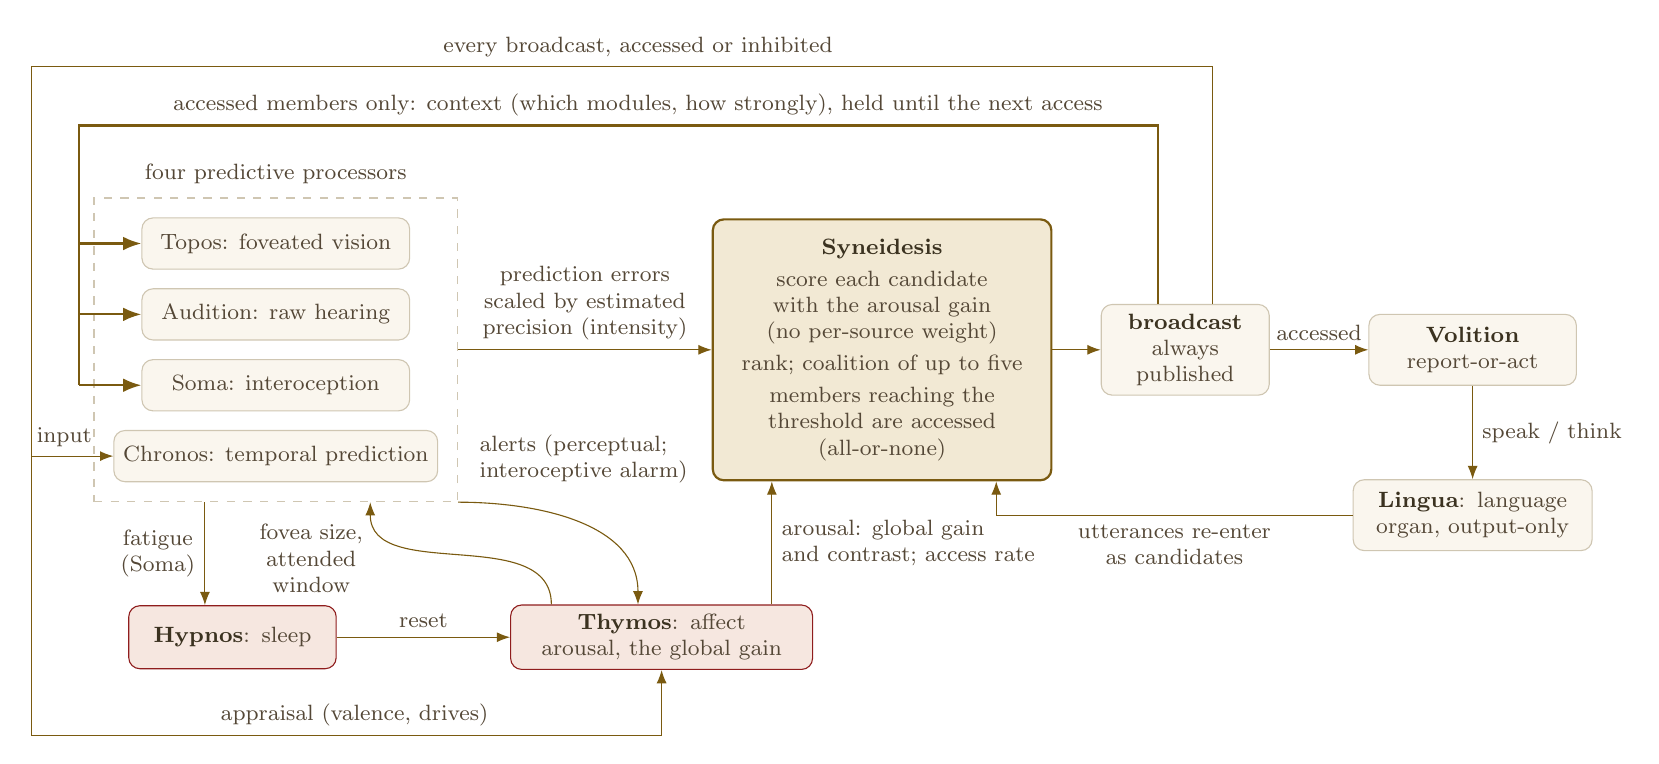
\begin{tikzpicture}[
  font=\small,>=Latex,
  every node/.append style={text=fgbody},
  every node/.append style={execute at begin node={\hyphenpenalty=10000\exhyphenpenalty=10000}},
  mod/.style={draw=bdim, rounded corners, fill=surf, align=center, minimum width=34mm, minimum height=6.5mm, font=\footnotesize},
  aff/.style={draw=bact, rounded corners, fill=surfact, align=center, minimum height=8mm, font=\footnotesize},
  work/.style={draw=bemph, thick, rounded corners, fill=surfemph, align=center, font=\footnotesize},
  act/.style={draw=bdim, rounded corners, fill=surf, align=center, minimum height=9mm, font=\footnotesize},
  lbl/.style={font=\footnotesize, text=fgbody, align=center},
]
% four predictive processors on the left
\node[mod] (m1) at (0,3.0) {Topos: foveated vision};
\node[mod] (m2) at (0,2.1) {Audition: raw hearing};
\node[mod] (m3) at (0,1.2) {Soma: interoception};
\node[mod] (m4) at (0,0.3) {Chronos: temporal prediction};
\node[draw=bdim, dashed, fit=(m1)(m2)(m3)(m4), inner sep=7pt] (mods) {};
\node[lbl, above=0.5mm of mods] {four predictive processors};
% workspace
\node[work, text width=38mm, inner sep=2.5mm] (syn) at (7.7,1.65)
  {\textcolor{fg}{\textbf{Syneidesis}}\\[2pt]
   score each candidate\\with the arousal gain\\(no per-source weight)\\[2pt]
   rank; coalition of up to five\\[2pt]
   members reaching the\\threshold are accessed\\(all-or-none)};
% broadcast
\node[mod, minimum width=0mm, text width=19mm, minimum height=11mm] (bc) at (11.55,1.65)
  {\textcolor{fg}{\textbf{broadcast}}\\\footnotesize always published};
% report path
\node[act, text width=24mm] (vol) at (15.2,1.65) {\textcolor{fg}{\textbf{Volition}}\\report-or-act};
\node[act, text width=28mm] (lin) at (15.2,-0.45) {\textcolor{fg}{\textbf{Lingua}}: language\\organ, output-only};
% affect and sleep below
\node[aff, text width=36mm] (thy) at (4.9,-2.0) {\textcolor{fg}{\textbf{Thymos}}: affect\\arousal, the global gain};
\node[aff, text width=24mm] (hyp) at (-0.55,-2.0) {\textcolor{fg}{\textbf{Hypnos}}: sleep};
% errors -> workspace
\draw[->, draw=stroke] (mods.east |- syn.west) -- node[lbl, above]{prediction errors\\scaled by estimated\\precision (intensity)} (syn.west);
% workspace -> broadcast -> volition -> lingua
\draw[->, draw=stroke] (syn.east) -- (bc.west);
\draw[->, draw=stroke] (bc.east) -- node[lbl, above]{accessed} (vol.west);
\draw[->, draw=stroke] (vol.south) -- node[lbl, right]{speak / think} (lin.north);
% utterances re-enter
\draw[->, draw=stroke] (lin.west) -- (9.15,-0.45) node[lbl, below, pos=0.5]{utterances re-enter\\as candidates} -- (9.15,0 |- syn.south);
% accessed broadcast -> prediction context of Topos, Audition, Soma
\coordinate (ctxa) at ($(bc.north)+(-0.35,0)$);
\coordinate (ctxt) at (0,4.5);
\draw[thick, draw=stroke] (ctxa) -- (ctxa |- ctxt) -- (-2.5,4.5) -- (-2.5,1.2);
\node[lbl, above] at (4.6,4.5) {accessed members only: context (which modules, how strongly), held until the next access};
\foreach \m in {m1,m2,m3} { \draw[->, thick, draw=stroke] (-2.5,0 |- \m.west) -- (\m.west); }
% every broadcast -> Chronos (input) and Thymos (appraisal)
\coordinate (evta) at ($(bc.north)+(0.35,0)$);
\coordinate (evtt) at (0,5.25);
\draw[draw=stroke] (evta) -- (evta |- evtt) -- (-3.1,5.25) -- (-3.1,-3.25) -- (4.9,-3.25);
\node[lbl, above] at (4.6,5.25) {every broadcast, accessed or inhibited};
\draw[->, draw=stroke] (-3.1,0 |- m4.west) -- node[lbl, above, font=\footnotesize, pos=0.4]{input} (m4.west);
\draw[->, draw=stroke] (4.9,-3.25) -- (thy.south);
\node[lbl, above] at (1.0,-3.25) {appraisal (valence, drives)};
% sleep and its reset
\draw[->, draw=stroke] (-0.9,0 |- mods.south) -- node[lbl, left]{fatigue\\(Soma)} (-0.9,0 |- hyp.north);
\draw[->, draw=stroke] (hyp.east) -- (thy.west);
\node[lbl, above] at ($(hyp.east)!0.5!(thy.west)$) {reset};
% alerts in, apertures out, arousal to selection
\draw[->, draw=stroke] (mods.south east) to[out=0,in=90] ($(thy.north)+(-0.3,0)$);
\node[lbl, anchor=south west, align=left] at ($(mods.south east)+(0.15,0.12)$) {alerts (perceptual;\\interoceptive alarm)};
\draw[->, draw=stroke] ($(thy.north)+(-1.4,0)$) to[out=90,in=-90]  (1.2,0 |- mods.south);
\node[lbl] at (0.45,-1.0) {fovea size,\\attended\\window};
\coordinate (aro) at ($(thy.north)+(1.4,0)$);
\draw[->, draw=stroke] (aro) -- node[lbl, right, align=left]{arousal: global gain\\and contrast; access rate} (aro |- syn.south);
\end{tikzpicture}
\end{document}
